%%%%%%%%%%%%%%%%%%%%%%%%%%%%%%%%%%%%%%%%%%%%%%
% To select a journal, use its code for the 
% journal= option in the \documentclass command.
% The journal codes for this template are:
% 
% Annals of Actuarial Science: aas
% British Journal of Political Science: jps
% Network Science: nws
% Political Analysis: pla
% Political Science Research and Methods: ram
% Evolutionary Human Sciences: ehs
% Natural Language Processing: nlp
%%%%%%%%%%%%%%%%%%%%%%%%%%%%%%%%%%%%%%%%%%%%%%
\documentclass[ 
  journal=medium,
  manuscript=article-type,
  year=2020,
  volume=37,
]{cup-journal}

\usepackage{amsmath}
\usepackage[nopatch]{microtype}
\usepackage{booktabs}

\title{Assignment 2: Data and methodology}

\author{Thomas Hoang / Student ID: A1984077}

\addbibresource{example.bib}

\keywords{keyword entry 1, keyword entry 2, keyword entry 3} %% First letter not capped

\begin{document}

\begin{abstract}
  Insert abstract text here. Lorem ipsum dolor sit amet, consectetur adipiscing elit, sed do eiusmod tempor incididunt ut labore et dolore magna aliqua. Lorem ipsum dolor sit amet, consectetur adipiscing elit, sed do eiusmod tempor incididunt ut labore et dolore magna aliqua. Lorem ipsum dolor sit amet, consectetur adipiscing elit, sed do eiusmod tempor incididunt ut labore et dolore magna aliqua.
\end{abstract}

\section{Introduction \& Related Work}

This demo file is intended to serve as a ``starter file''. It is for preparing manuscript submission only, not for preparing camera-ready versions of manuscripts. Manuscripts will be typeset for publication by the journal, after they have been accepted.

By default, this template uses \texttt{biblatex} and adopts the Chicago referencing style. However, the journal you’re submitting to may require a different reference style; specify the journal you're using with the class' \texttt{journal} option --- see lines 1--13 of \emph{sample.tex} for a list of options and instructions for selecting the journal. If you are using this template on Overleaf, Overleaf's build tool will automatically run \texttt{pdflatex} and \texttt{biber}. If you are compiling this template on your own local \LaTeX{} installation, please execute the following commands:
\begin{enumerate}
  \item \verb|pdflatex sample|
  \item \verb|biber sample|
  \item \verb|pdflatex sample|
  \item \verb|pdflatex sample|
\end{enumerate}

Lorem ipsum dolor sit amet, consectetur adipiscing elit, sed do eiusmod tempor incididunt ut labore et dolore magna aliqua.

Lorem ipsum dolor sit amet, consectetur adipiscing elit, sed do eiusmod tempor incididunt ut labore et dolore magna aliqua. Lorem ipsum dolor sit amet, consectetur adipiscing elit, sed do eiusmod tempor incididunt ut labore et dolore magna aliqua.


\subsection{sdf}
Subsection text here. Lorem ipsum\autocite{Bayer_etal_2013} dolor sit amet, consectetur adipiscing elit, sed do eiusmod tempor incididunt ut labore\autocite{Adade_etal_2007} et dolore magna aliqua.

Lorem ipsum dolor sit amet, consectetur adipiscing elit, sed do eiusmod tempor incididunt ut labore et dolore magna aliqua. Lorem ipsum dolor sit amet, consectetur adipiscing elit, sed do eiusmod tempor incididunt ut labore et dolore magna aliqua. Lorem ipsum dolor sit amet, consectetur adipiscing elit, sed do eiusmod tempor incididunt ut labore et dolore magna aliqua.

\subsubsection{sgsdfs}
Subsubsection text here. Lorem ipsum dolor sit amet, consectetur adipiscing elit, sed do eiusmod tempor incididunt ut labore et dolore magna aliqua.
Lorem ipsum dolor sit amet, consectetur adipiscing elit, sed do eiusmod tempor incididunt ut labore et dolore magna aliqua.

Lorem ipsum dolor sit amet, consectetur adipiscing elit, sed do eiusmod tempor incididunt ut labore et dolore magna aliqua. Lorem ipsum dolor sit amet, consectetur adipiscing elit, sed do\endnote{A footnote/endnote} eiusmod tempor incididunt ut labore et dolore magna aliqua.

\section{Dataset, Data Preparation \& Architecture Design}

\subsection{Dataset Description}
The dataset was sourced from the internal \texttt{\textbf{Staging}} database, which contains sufficient \textbf{real-world sales-call data} used in our product operations. Data extraction was performed with \textbf{SQL} using the following query:

\begin{verbatim}
SELECT * from call_call WHERE type='MANUAL' and record != '' and duration > 5 
ORDER BY created_at DESC;
\end{verbatim}

The condition \texttt{\textbf{duration > 5}} was applied to ensure the call actually took place and to filter out very short or invalid records. The query output was exported to a \textbf{CSV} file, resulting in a final dataset of \textbf{13{,}232 records}.

\subsection{Data Visualization}
To inspect recording quality and segmentation behavior, we visualized the temporal structure of the audio before and after preprocessing. Figure~\ref{fig_dataset_viz} illustrates a waveform-style view where low-amplitude regions correspond to silence and higher-energy regions correspond to active speech.

\begin{figure}[hbt!]
  \centering
  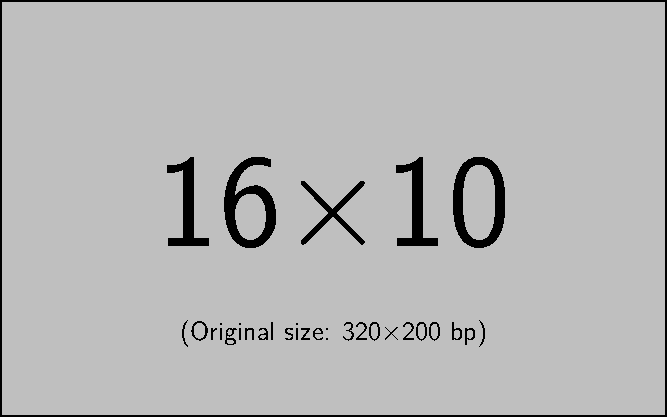
\includegraphics[width=0.85\linewidth]{example-image-16x10.pdf}
  \caption{Example audio visualization (waveform/energy profile) highlighting silence and speech intervals used in segmentation analysis.}
  \label{fig_dataset_viz}
\end{figure}

In addition to waveform plots, a duration histogram can be used to compare chunk lengths before and after Voice Activity Detection (VAD), showing that long silence-heavy segments are split into shorter speech-focused chunks.

\subsection{Pre-processing Step 1: Voice Activity Detection (VAD)}
The first preprocessing stage applies Silero VAD to remove non-speech regions and split each call into speech segments. Silero VAD is designed for low-latency inference and can process short audio windows (30+ ms chunks) in under 1 ms on modern hardware. This makes it suitable for large-scale batch pipelines and near-real-time settings.

For implementation flexibility, Silero VAD supports both PyTorch and ONNX backends. In this project, the backend choice depends on the deployment target: PyTorch for rapid experimentation and ONNX for optimized inference portability.

\subsection{Pre-processing Step 2: Speech-to-Text (ASR)}
After VAD segmentation, each speech-only chunk is forwarded to an Automatic Speech Recognition (ASR) model (e.g., Qwen3-ASR). The ASR model converts audio segments into unstructured text transcripts while preserving conversational order. Segment-level transcripts are then merged chronologically to reconstruct each full-call transcript.

\subsection{Ground Truth Dataset Creation (Step 3)}
In the final stage, reconstructed transcripts are transformed into instruction-tuning samples for LLM fine-tuning. Each sample is formatted as an \texttt{Instruction/Response} pair in JSON, where the instruction defines the task (e.g., summarize the call, extract customer intent, detect objections) and the response provides the expected target output.

A simplified record format is shown below:
\begin{verbatim}
{
  "instruction": "Summarize the sales call and list key objections.",
  "input": "<full transcript text>",
  "response": "<structured summary and objection list>"
}
\end{verbatim}

This schema standardizes supervision signals and produces a clean ground-truth dataset for supervised fine-tuning of the downstream LLM.


\section{Deep Learning Methodology}

The output for a single-column figure is in Figure~\ref{fig_sim}.  Lorem ipsum dolor sit amet, consectetur adipiscing elit, sed do eiusmod tempor incididunt ut labore et dolore magna aliqua. Lorem ipsum dolor sit amet, consectetur adipiscing elit, sed do eiusmod tempor incididunt ut labore et dolore magna aliqua. Lorem ipsum dolor sit amet, consectetur adipiscing elit, sed do eiusmod tempor incididunt ut labore et dolore magna aliqua.

Lorem ipsum dolor sit amet, consectetur adipiscing elit, sed do eiusmod tempor incididunt ut labore et dolore magna aliqua. Lorem ipsum dolor sit amet, consectetur adipiscing elit, sed do eiusmod tempor incididunt ut labore et dolore magna aliqua. Lorem ipsum dolor sit amet, consectetur adipiscing elit, sed do eiusmod tempor incididunt ut labore et dolore magna aliqua.

%See Figure~\ref{fig_wide} for a double-column figure; this is always at the top of a following page.


\begin{figure}[hbt!]
  \centering
  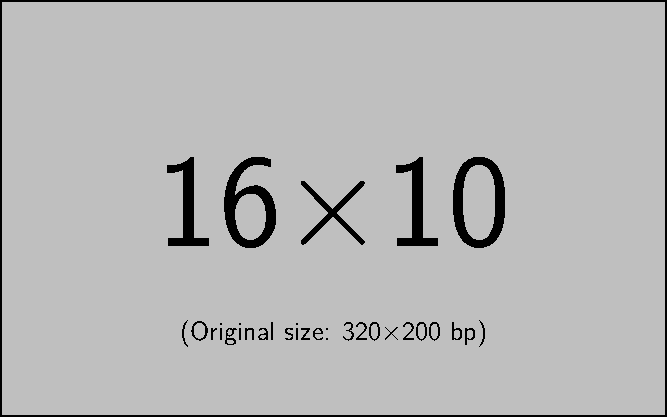
\includegraphics[width=0.75\linewidth]{example-image-16x10.pdf}
  \caption{Insert figure caption here}
  \label{fig_sim}
\end{figure}


\begin{figure*}
  \centering
  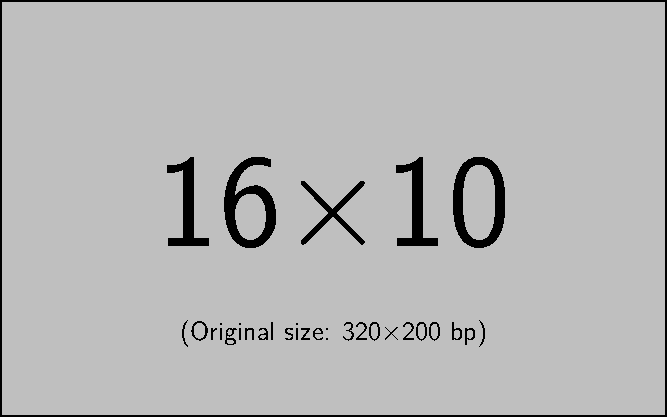
\includegraphics[width=0.8\linewidth]{example-image-16x10.pdf}
  \caption{Insert figure caption here}
  \label{fig_wide}
\end{figure*}


See example table in Table~\ref{table_example}.

\begin{table}[hbt!]
  \begin{threeparttable}
    \caption{An Example of a Table}
    \label{table_example}
    \begin{tabular}{llll}
      \toprule
      \headrow Column head 1 & Column head 2 & Column head 3        & Column head 4 \\
      \midrule
      One\tnote{a}           & Two           & three three          & four          \\
      \midrule
      Three                  & Four          & three three\tnote{b} & four          \\
      \bottomrule
    \end{tabular}
    \begin{tablenotes}[hang]
      \item[]Table note
      \item[a]First note
      \item[b]Another table note
    \end{tablenotes}
  \end{threeparttable}
\end{table}


\section{Evaluation Metrics}
The conclusion text goes here.


\paragraph{Acknowledgments}
We are grateful for the technical assistance of A. Author.


\paragraph{Funding Statement}
This research was supported by grants from the <funder-name><doi>(<award ID>); <funder-name><doi>(<award ID>).

\paragraph{Competing Interests}
A statement about any financial, professional, contractual or personal relationships or situations that could be perceived to impact the presentation of the work --- or `None' if none exist

\paragraph{Data Availability Statement}
A statement about how to access data, code and other materials allowing users to understand, verify and replicate findings --- e.g. Replication data and code can be found in Harvard Dataverse: \verb+\url{https://doi.org/link}+.

\paragraph{Ethical Standards}
The research meets all ethical guidelines, including adherence to the legal requirements of the study country.

\paragraph{Author Contributions}
Please provide an author contributions statement using the CRediT taxonomy roles as a guide {\verb+\url{https://www.casrai.org/credit.html}+}. Conceptualization: A.A; A.B. Methodology: A.A; A.B. Data curation: A.C. Data visualisation: A.C. Writing original draft: A.A; A.B. All authors approved the final submitted draft.


%\endnote in some journals will behave like \footnote; and \printendnotes will not output anything. 
\printendnotes

\defbibnote{preamble}{By default, this template uses \texttt{biblatex} and adopts the Chicago referencing style. However, the journal you’re submitting to may require a different reference style; specify the journal you're using with the class' \texttt{journal} option --- see lines 1--13 of \emph{sample.tex} for a list of options and instructions for selecting the journal.}

\printbibliography[prenote={preamble}]
\appendix

\section{Example Appendix Section}

Lorem ipsum dolor sit amet, consectetur adipiscing elit, sed do eiusmod tempor incididunt ut labore et dolore magna aliqua. Lorem ipsum dolor sit amet, consectetur adipiscing elit, sed do eiusmod tempor incididunt ut labore et dolore magna aliqua. Lorem ipsum dolor sit amet, consectetur adipiscing elit, sed do eiusmod tempor incididunt ut labore et dolore magna aliqua.

\end{document}